\documentclass[utf8x]{beamer}

% This file is a solution template for:

% - Talk at a conference/colloquium.
% - Talk length is about 20min.
% - Style is ornate.

\mode<presentation>
{
  \usetheme{Warsaw}
  % or ...

  %\setbeamercovered{transparent}
  % or whatever (possibly just delete it)
}


\usepackage[english]{babel}
\usepackage{listings}
\usepackage{ulem}
\usepackage{color}
\usepackage{alltt}

\usepackage[utf8x]{inputenc}


\newcommand\redsout[1]{{\color{red}\sout{\hbox{\color{black}{#1}}}}}

% or whatever

% Or whatever. Note that the encoding and the font should match. If T1
% does not look nice, try deleting the line with the fontenc.


\title{The Efficient Handling of Guards in the Design of RPython's Tracing JIT}

\author[David Schneider, Carl Friedrich Bolz]{David Schneider \and \emph{Carl Friedrich Bolz}}
% - Give the names in the same order as the appear in the paper.
% - Use the \inst{?} command only if the authors have different
%   affiliation.

\institute[Heinrich-Heine-Universität Düsseldorf]{
Heinrich-Heine-Universität Düsseldorf, STUPS Group, Germany
}

\date{2012 VMIL, 21st of October, 2012}
% - Either use conference name or its abbreviation.
% - Not really informative to the audience, more for people (including
%   yourself) who are reading the slides online


% If you have a file called "university-logo-filename.xxx", where xxx
% is a graphic format that can be processed by latex or pdflatex,
% resp., then you can add a logo as follows:




% Delete this, if you do not want the table of contents to pop up at
% the beginning of each subsection:
%\AtBeginSubsection[]
%{
%  \begin{frame}<beamer>
%    \frametitle{Outline}
%    \tableofcontents[currentsection,currentsubsection]
%  \end{frame}
%}


% If you wish to uncover everything in a step-wise fashion, uncomment
% the following command:

%\beamerdefaultoverlayspecification{<+->}


\begin{document}

\begin{frame}
  \titlepage
\end{frame}

\section{Introduction}

\begin{frame}
  \frametitle{Tracing JITs Compile by Observing an Interpreter}
  \begin{itemize}
      \item VM contains both an interpreter and the tracing JIT compiler
      \item JIT works by observing and logging what the interpreter does
      \begin{itemize}
          \item for interesting, commonly executed code paths
          \item produces a linear list of operations (trace)
          \item automatically does (potentially deep) inlining
      \end{itemize}
      \item trace is optimized and then turned into machine code
  \end{itemize}
\end{frame}

\begin{frame}
  \frametitle{Guards}
  \begin{itemize}
      \item Points of control flow divergence are marked with guards
      \item Operations that check whether conditions are still true
      \item When a guard fails, execution of the trace stops and continues in the interpreter
      \pause
      \begin{block}{Guard Characteristics}
          \begin{itemize}
              \item lots of them, up to 20\% guards
              \item most never fail
              \item costly to implement
          \end{itemize}
      \end{block}
  \end{itemize}
\end{frame}

% this talk wants to go over a lot of details that are usually glossed over as
% "easy" when tracing JITs are introduced.

\begin{frame}
  \frametitle{Bridges}
  \begin{itemize}
      \item When a trace fails often, it becomes worth to attach a new trace to it
          \item This is called a bridge
          \item The bridge is attached by patching the guard machine code
          \item when this guard fails in the future, the new trace is executed instead
  \end{itemize}
\end{frame}

\begin{frame}
  \frametitle{RPython and PyPy}
  \begin{itemize}
      \item Context: RPython
      \item a generic tracing JIT, applicable to many languages
      \item main use: PyPy, an efficient Python interpreter
  \end{itemize}
\end{frame}

\begin{frame}
  \frametitle{Running Example}
\end{frame}

\section{High-Level}

\begin{frame}
  \frametitle{Symbolic Frame Capturing}
  \begin{itemize}
      \item Guard can fail deep inside inlined function
      \item when going back to the interpreter, call stack needs to be re-created
      \item done with the help of symbolic frame stacks
      \item these show how trace variables fill the to-be-built stack frames
  \end{itemize}
\end{frame}

\begin{frame}
  \frametitle{Symbolic Frame Compression}
  \begin{itemize}
      \item There are \emph{a lot of} guards
      \item Naively storing symbolic frames would be costly in terms of memory
      \item need to store them compactly
      \item observation: from one guard to the next, the non-top stack frames don't change
      \item share these between subsequent guards
      \pause
      \item also need a byte-saving binary representation, but that's just boring work
  \end{itemize}
\end{frame}

\begin{frame}
  \frametitle{Interaction with Optimization}
  \begin{itemize}
      \item Some optimizations make it necessary to store extra information in symbolic frames
      \item examples:
          \begin{itemize}
              \item delayed heap stores (need to do stores before resuming interpreter)
              \item allocation removal (need to allocate objects before resuming)
          \end{itemize}
      \item can be compressed using similar techniques
  \end{itemize}
\end{frame}

\begin{frame}
  \frametitle{Emitting Guards}
\end{frame}

\begin{frame}
  \begin{figure}
  \centering
  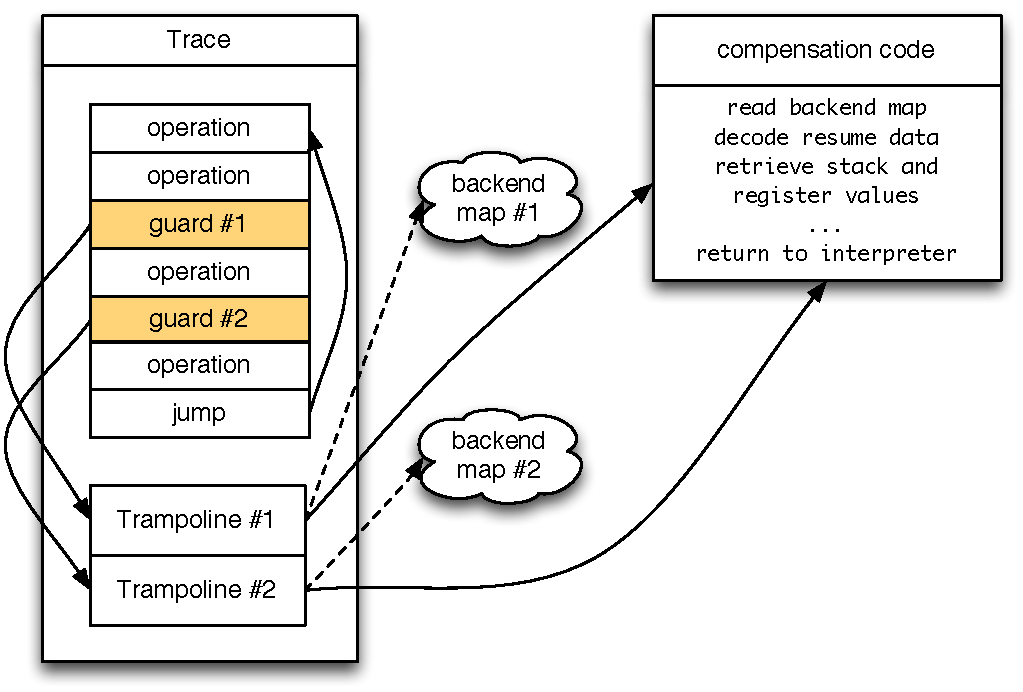
\includegraphics[width=1\textwidth]{figures/loop.pdf}
  \label{fig:trampoline}
  \end{figure}
\end{frame}

\begin{frame}
  \begin{figure}
  \centering
  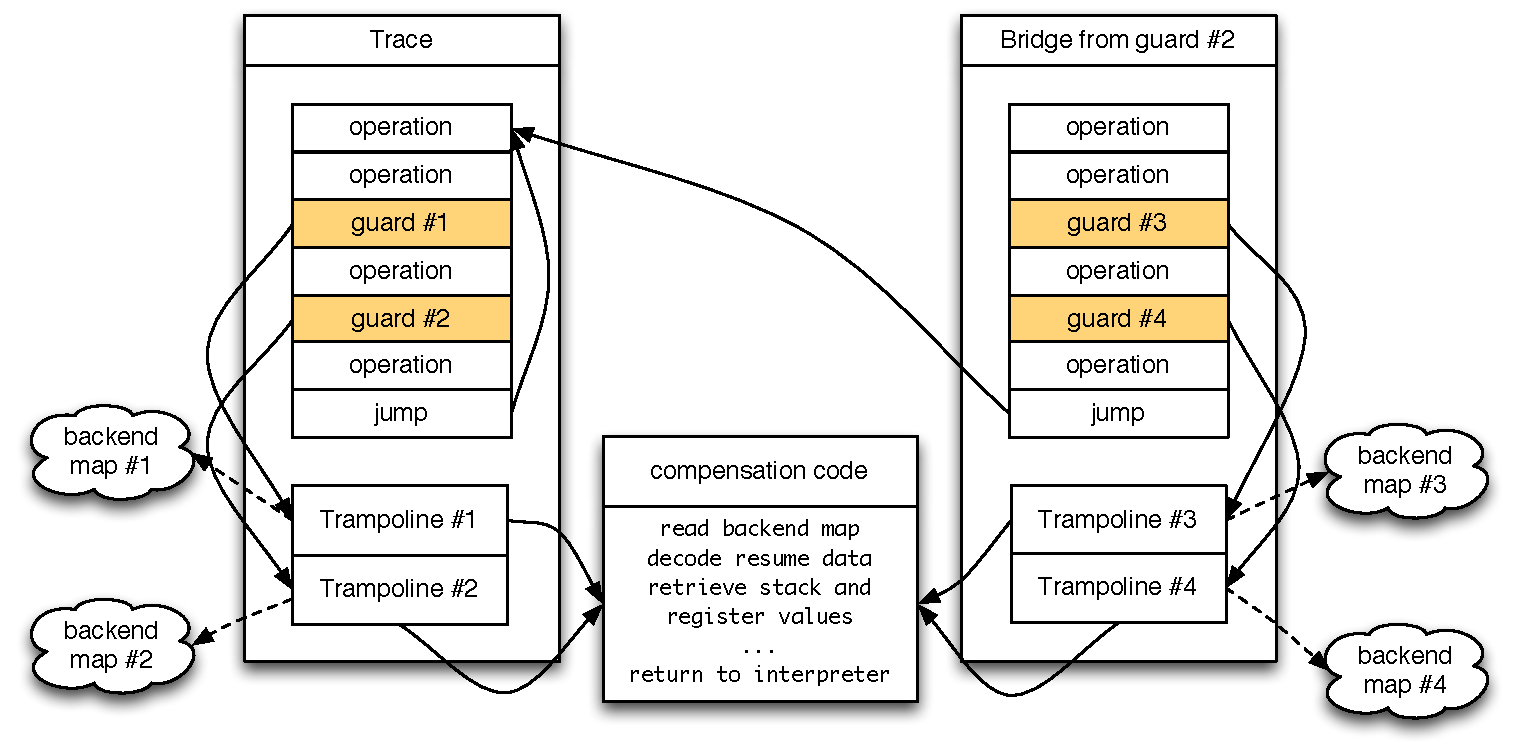
\includegraphics[width=1\textwidth]{figures/bridge_compiled.pdf}
  \label{fig:trampoline}
  \end{figure}
\end{frame}
\begin{frame}
  \begin{figure}
  \centering
  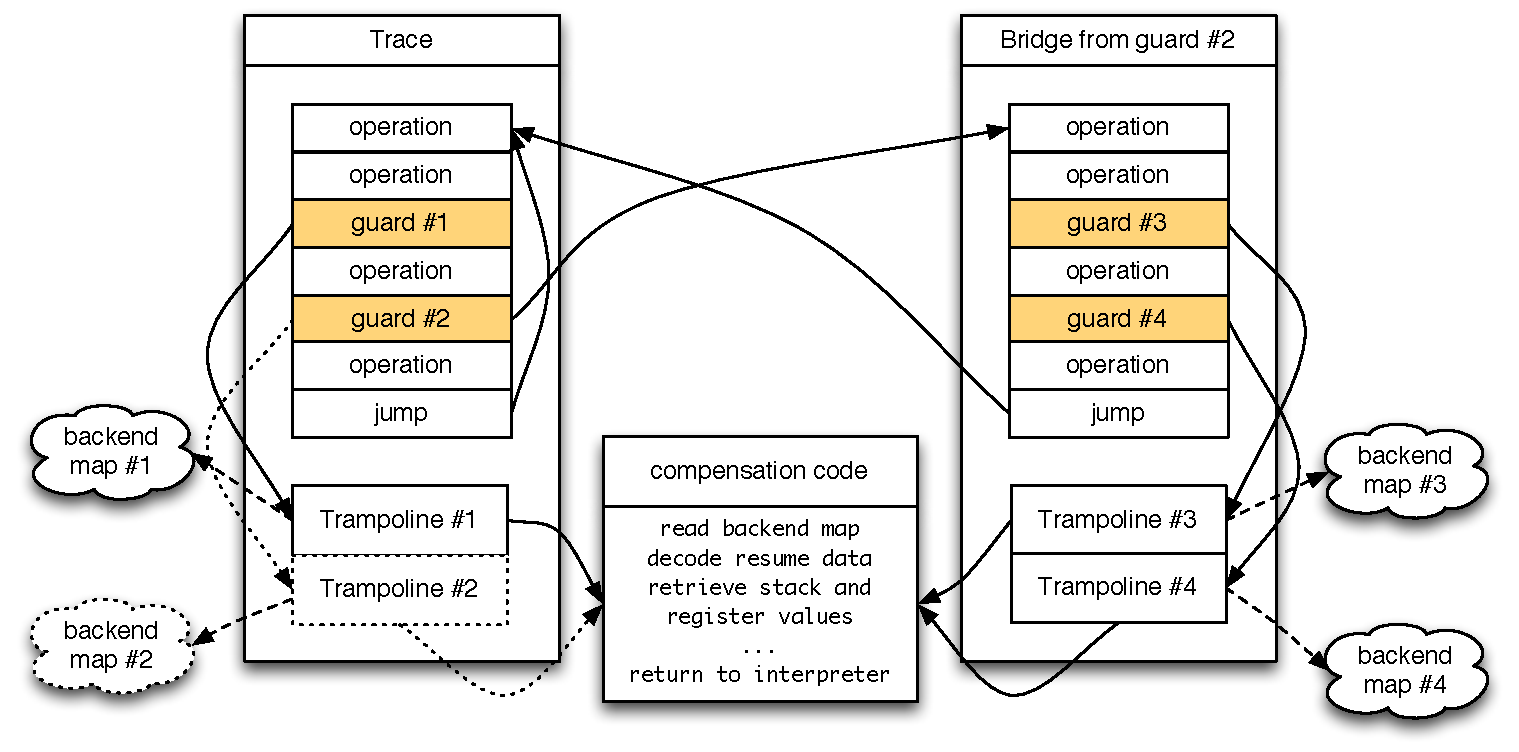
\includegraphics[width=1\textwidth]{figures/bridge_patched.pdf}
  \label{fig:trampoline}
  \end{figure}
\end{frame}

\begin{frame}
  \frametitle{Patching Guards for Bridges}
\end{frame}

\section{Evaluation}

%as in paper
%fancy graphs
%something about execution speed
% <demo, if there is time>
\end{document}
